\chapter{Piles et électrolyse}\label{ch:g12:cells-and-electrolysis}

Un soir d'hiver, un téléphone affiche 1~\% puis s'éteint. Branché toute
la nuit, il est de nouveau chargé au matin. Dans sa batterie, la même
\omterm{def:g7:chemical-reactions:reaction}{réaction chimique} se déroule dans un sens pendant la journée, en
fournissant de l'énergie électrique, et elle est forcée dans l'autre
sens pendant la nuit par le chargeur. Une \omterm{def:g11:redox:reaction}{réaction d'oxydoréduction}
devient une source d'électricité quand on oblige ses \omterm{def:g9:inside-the-atom:nucleus}{électrons} à
parcourir un fil~; et l'électricité, imposée à travers une solution,
peut forcer une \omterm{def:g11:redox:reaction}{réaction d'oxydoréduction} qui ne se produirait jamais
d'elle-même.

\begin{recall}
Les \omterm{def:g11:redox:oxidant}{oxydants} gagnent des \omterm{def:g9:inside-the-atom:nucleus}{électrons}, les \omterm{def:g11:redox:oxidant}{réducteurs} en perdent~;
\omterm{def:g11:redox:couple}{demi-équations}, \omterm{def:g11:redox:couple}{couples oxydant/réducteur} et \omterm{def:g11:redox:reaction}{réactions
d'oxydoréduction} (\cref{ch:g11:redox}). Un système évolue jusqu'à ce
que
$Q = K$ (\cref{ch:g12:equilibrium}). Les solutions ioniques conduisent
le courant (\cref{ch:g9:ions})~; la \omterm{def:g10:the-mole:amount}{mole} et la \omterm{def:g10:the-mole:avogadro}{constante d'Avogadro}
(\cref{ch:g10:the-mole}).
\end{recall}

\begin{omfigure}
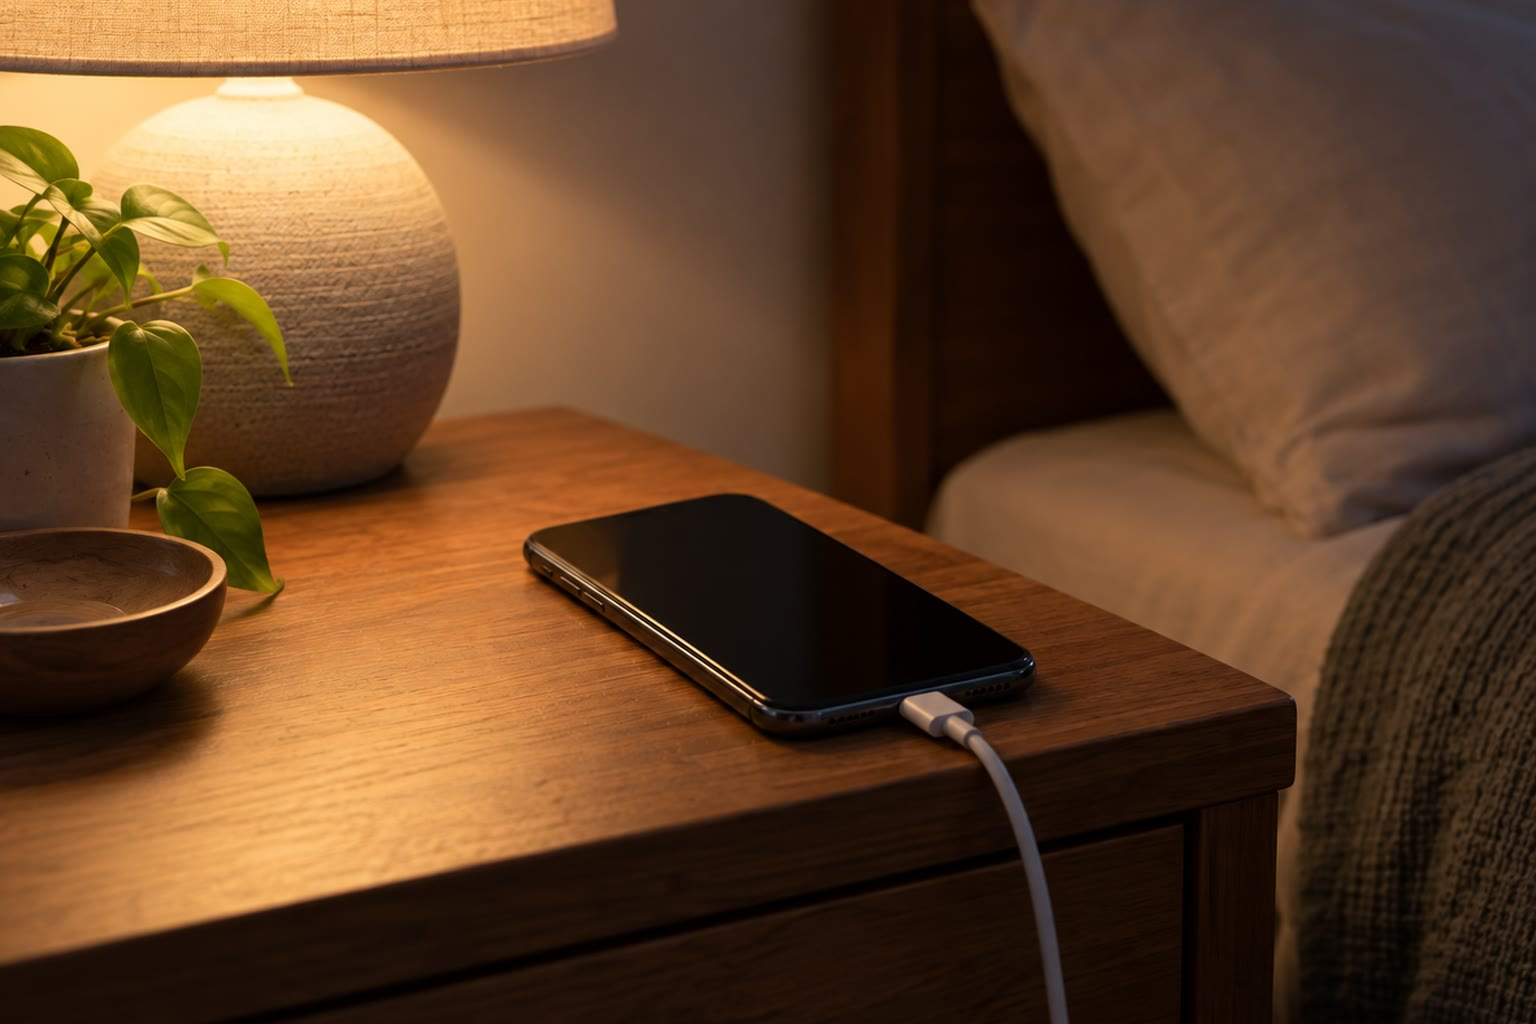
\includegraphics[width=0.45\linewidth]{images/book1/ai/g12-phone-charging.jpg}

{\small Recharger un téléphone~: une réaction forcée en sens inverse
pendant la nuit.}
\end{omfigure}

\section{Une réaction d'oxydoréduction coupée en deux}

Quand on plonge une lame de zinc dans une solution de sulfate de
cuivre, le zinc est oxydé et les \omterm{def:g9:ions:ion}{ions} cuivre sont réduits à la surface
de la lame,
\ce{Zn + Cu^{2+} -> Zn^{2+} + Cu}~: les \omterm{def:g9:inside-the-atom:nucleus}{électrons} passent directement du
\omterm{def:g9:periodic-table-first-look:metal}{métal} aux \omterm{def:g9:ions:ion}{ions}, et l'énergie est perdue sous forme d'un peu de chaleur.
Séparons les deux moitiés et relions-les par un fil~: les \omterm{def:g9:inside-the-atom:nucleus}{électrons}
doivent alors parcourir le fil, et peuvent allumer une lampe au passage.

\begin{definition}[Pile, demi-pile, pont salin]\label{def:g12:cells-and-electrolysis:cell}
Une \emph{pile}\index{pile} produit de l'énergie électrique à partir
d'une \omterm{def:g11:redox:reaction}{réaction d'oxydoréduction} dont l'\omterm{def:g11:redox:oxidation}{oxydation} et la \omterm{def:g11:redox:oxidation}{réduction} ont
lieu dans deux compartiments séparés. Chaque compartiment, une électrode
métallique plongeant dans une solution de ses \omterm{def:g9:ions:ion}{ions}, est une
\emph{demi-pile}\index{demi-pile}. Un \emph{pont salin}\index{pont salin},
tube ou bande de papier imbibés d'une solution ionique, relie les deux
solutions et ferme le circuit tout en les maintenant séparées.
\end{definition}

\begin{definition}[Anode, cathode]\label{def:g12:cells-and-electrolysis:anode}
L'électrode où a lieu une \omterm{def:g11:redox:oxidation}{oxydation} est l'\emph{anode}\index{anode}~;
l'électrode où a lieu une \omterm{def:g11:redox:oxidation}{réduction} est la
\emph{cathode}\index{cathode}.
\end{definition}

\begin{omfigure}
\begin{tikzpicture}[font=\small, scale=1.25]
  \pic[transform shape] at (0,0) {beaker={0.7}{black!6}};
  \pic[transform shape] at (4,0) {beaker={0.7}{cyan!70!blue!35}};
  \pic[transform shape] (zn) at (-0.3,0.25) {electrode={black!30}};
  \pic[transform shape] (cu) at (4.3,0.25) {electrode={orange!70!brown}};
  \pic[transform shape] at (0.35,0.6) {saltbridge={3.3}};
  \pic[transform shape] (v) at (2,3.9) {meter={1.10 V}};
  \draw[black!70, thick] (zn-top) |- (1.0,3.4) -| (v-a);
  \draw[black!70, thick] (cu-top) |- (3.0,3.4) -| (v-b);
  \draw[->, omProp, very thick] (0.2,3.55) -- (1.0,3.55);
  \draw[->, omProp, very thick] (3.0,3.55) -- (3.8,3.55);
  \node[omProp, font=\footnotesize] at (0.6,3.75) {$e^-$};
  \node[omProp, font=\footnotesize] at (3.4,3.75) {$e^-$};
  \node[anchor=north, align=center] at (-0.2,-0.15) {anode ($-$)~: zinc\\ \ce{Zn -> Zn^{2+} + 2e-}};
  \node[anchor=north, align=center] at (4.2,-0.15) {cathode ($+$)~: cuivre\\ \ce{Cu^{2+} + 2e- -> Cu}};
  \node[font=\footnotesize, anchor=east, align=right] at (-0.95,0.7) {\ce{Zn^{2+}}\\ \ce{SO4^{2-}}};
  \node[font=\footnotesize, anchor=west, align=left] at (4.95,0.7) {\ce{Cu^{2+}}\\ \ce{SO4^{2-}}};
  \node[font=\footnotesize, align=center] at (2,2.45) {pont salin\\ (\ce{K+}, \ce{NO3-})};
\end{tikzpicture}

{\small La \omterm{def:g12:cells-and-electrolysis:cell}{pile} Daniell. Les \omterm{def:g9:inside-the-atom:nucleus}{électrons} quittent l'\omterm{def:g12:cells-and-electrolysis:anode}{anode} de zinc par le
fil et entrent dans la \omterm{def:g12:cells-and-electrolysis:anode}{cathode} de cuivre~; dans le \omterm{def:g12:cells-and-electrolysis:cell}{pont salin}, des \omterm{def:g9:ions:ion}{ions}
se déplacent pour maintenir chaque solution électriquement neutre.}
\end{omfigure}

\begin{proposition}[Où vont les électrons]\label{prop:g12:cells-and-electrolysis:flow}
Dans une \omterm{def:g12:cells-and-electrolysis:cell}{pile} qui débite, les \omterm{def:g9:inside-the-atom:nucleus}{électrons} sortent de la \omterm{def:g12:cells-and-electrolysis:cell}{pile} par l'\omterm{def:g12:cells-and-electrolysis:anode}{anode},
où l'\omterm{def:g11:redox:oxidation}{oxydation} les libère, parcourent le circuit extérieur, et entrent
par la \omterm{def:g12:cells-and-electrolysis:anode}{cathode}, où la \omterm{def:g11:redox:oxidation}{réduction} les capte. L'\omterm{def:g12:cells-and-electrolysis:anode}{anode} est la borne
négative, la \omterm{def:g12:cells-and-electrolysis:anode}{cathode} la borne positive. À l'intérieur, le courant est
assuré par les \omterm{def:g9:ions:ion}{ions}~: les \omterm{def:g9:ions:ion}{cations} se déplacent vers la \omterm{def:g12:cells-and-electrolysis:anode}{cathode}, les
\omterm{def:g9:ions:ion}{anions} vers l'\omterm{def:g12:cells-and-electrolysis:anode}{anode}.
\end{proposition}

\begin{proof}
L'\omterm{def:g11:redox:oxidation}{oxydation} produit des \omterm{def:g9:inside-the-atom:nucleus}{électrons} à l'\omterm{def:g12:cells-and-electrolysis:anode}{anode}~; la \omterm{def:g11:redox:oxidation}{réduction} les consomme
à la \omterm{def:g12:cells-and-electrolysis:anode}{cathode}~; le fil est le seul chemin entre les deux. Sinon, chaque
solution se chargerait électriquement, ce qu'empêchent les \omterm{def:g9:ions:ion}{ions} du pont.
\end{proof}

\begin{method}[Décrire une pile]\label{met:g12:cells-and-electrolysis:describe}
\begin{enumerate}
  \item Écrire la \omterm{def:g11:redox:reaction}{réaction d'oxydoréduction} globale qui se produit
        spontanément.
  \item La décomposer en deux \omterm{def:g11:redox:couple}{demi-équations}~: l'\omterm{def:g11:redox:oxidation}{oxydation} (\omterm{def:g12:cells-and-electrolysis:anode}{anode}) et la
        \omterm{def:g11:redox:oxidation}{réduction} (\omterm{def:g12:cells-and-electrolysis:anode}{cathode}).
  \item Indiquer la polarité~: \omterm{def:g12:cells-and-electrolysis:anode}{anode} $-$, \omterm{def:g12:cells-and-electrolysis:anode}{cathode} $+$~; le sens des
        \omterm{def:g9:inside-the-atom:nucleus}{électrons} dans le fil (de l'\omterm{def:g12:cells-and-electrolysis:anode}{anode} vers la \omterm{def:g12:cells-and-electrolysis:anode}{cathode}) et celui du
        courant (de la \omterm{def:g12:cells-and-electrolysis:anode}{cathode} vers l'\omterm{def:g12:cells-and-electrolysis:anode}{anode}).
  \item Décrire le mouvement des \omterm{def:g9:ions:ion}{ions} dans le pont.
\end{enumerate}
\end{method}


\begin{history}[La pile de Volta, 1800]
En 1800, le physicien Alessandro Volta empila des disques de deux
métaux différents, zinc et cuivre ou argent, séparés par des morceaux de
tissu imbibés d'eau salée, et obtint un courant électrique continu~: la
première \omterm{def:g12:cells-and-electrolysis:cell}{pile}. Elle donna aux physiciens leur première source continue
d'électricité, et aux chimistes un nouvel outil~: en quelques années,
l'\omterm{def:g12:cells-and-electrolysis:electrolysis}{électrolyse} permit d'isoler pour la première fois le sodium et le
potassium.
\end{history}

\begin{omfigure}
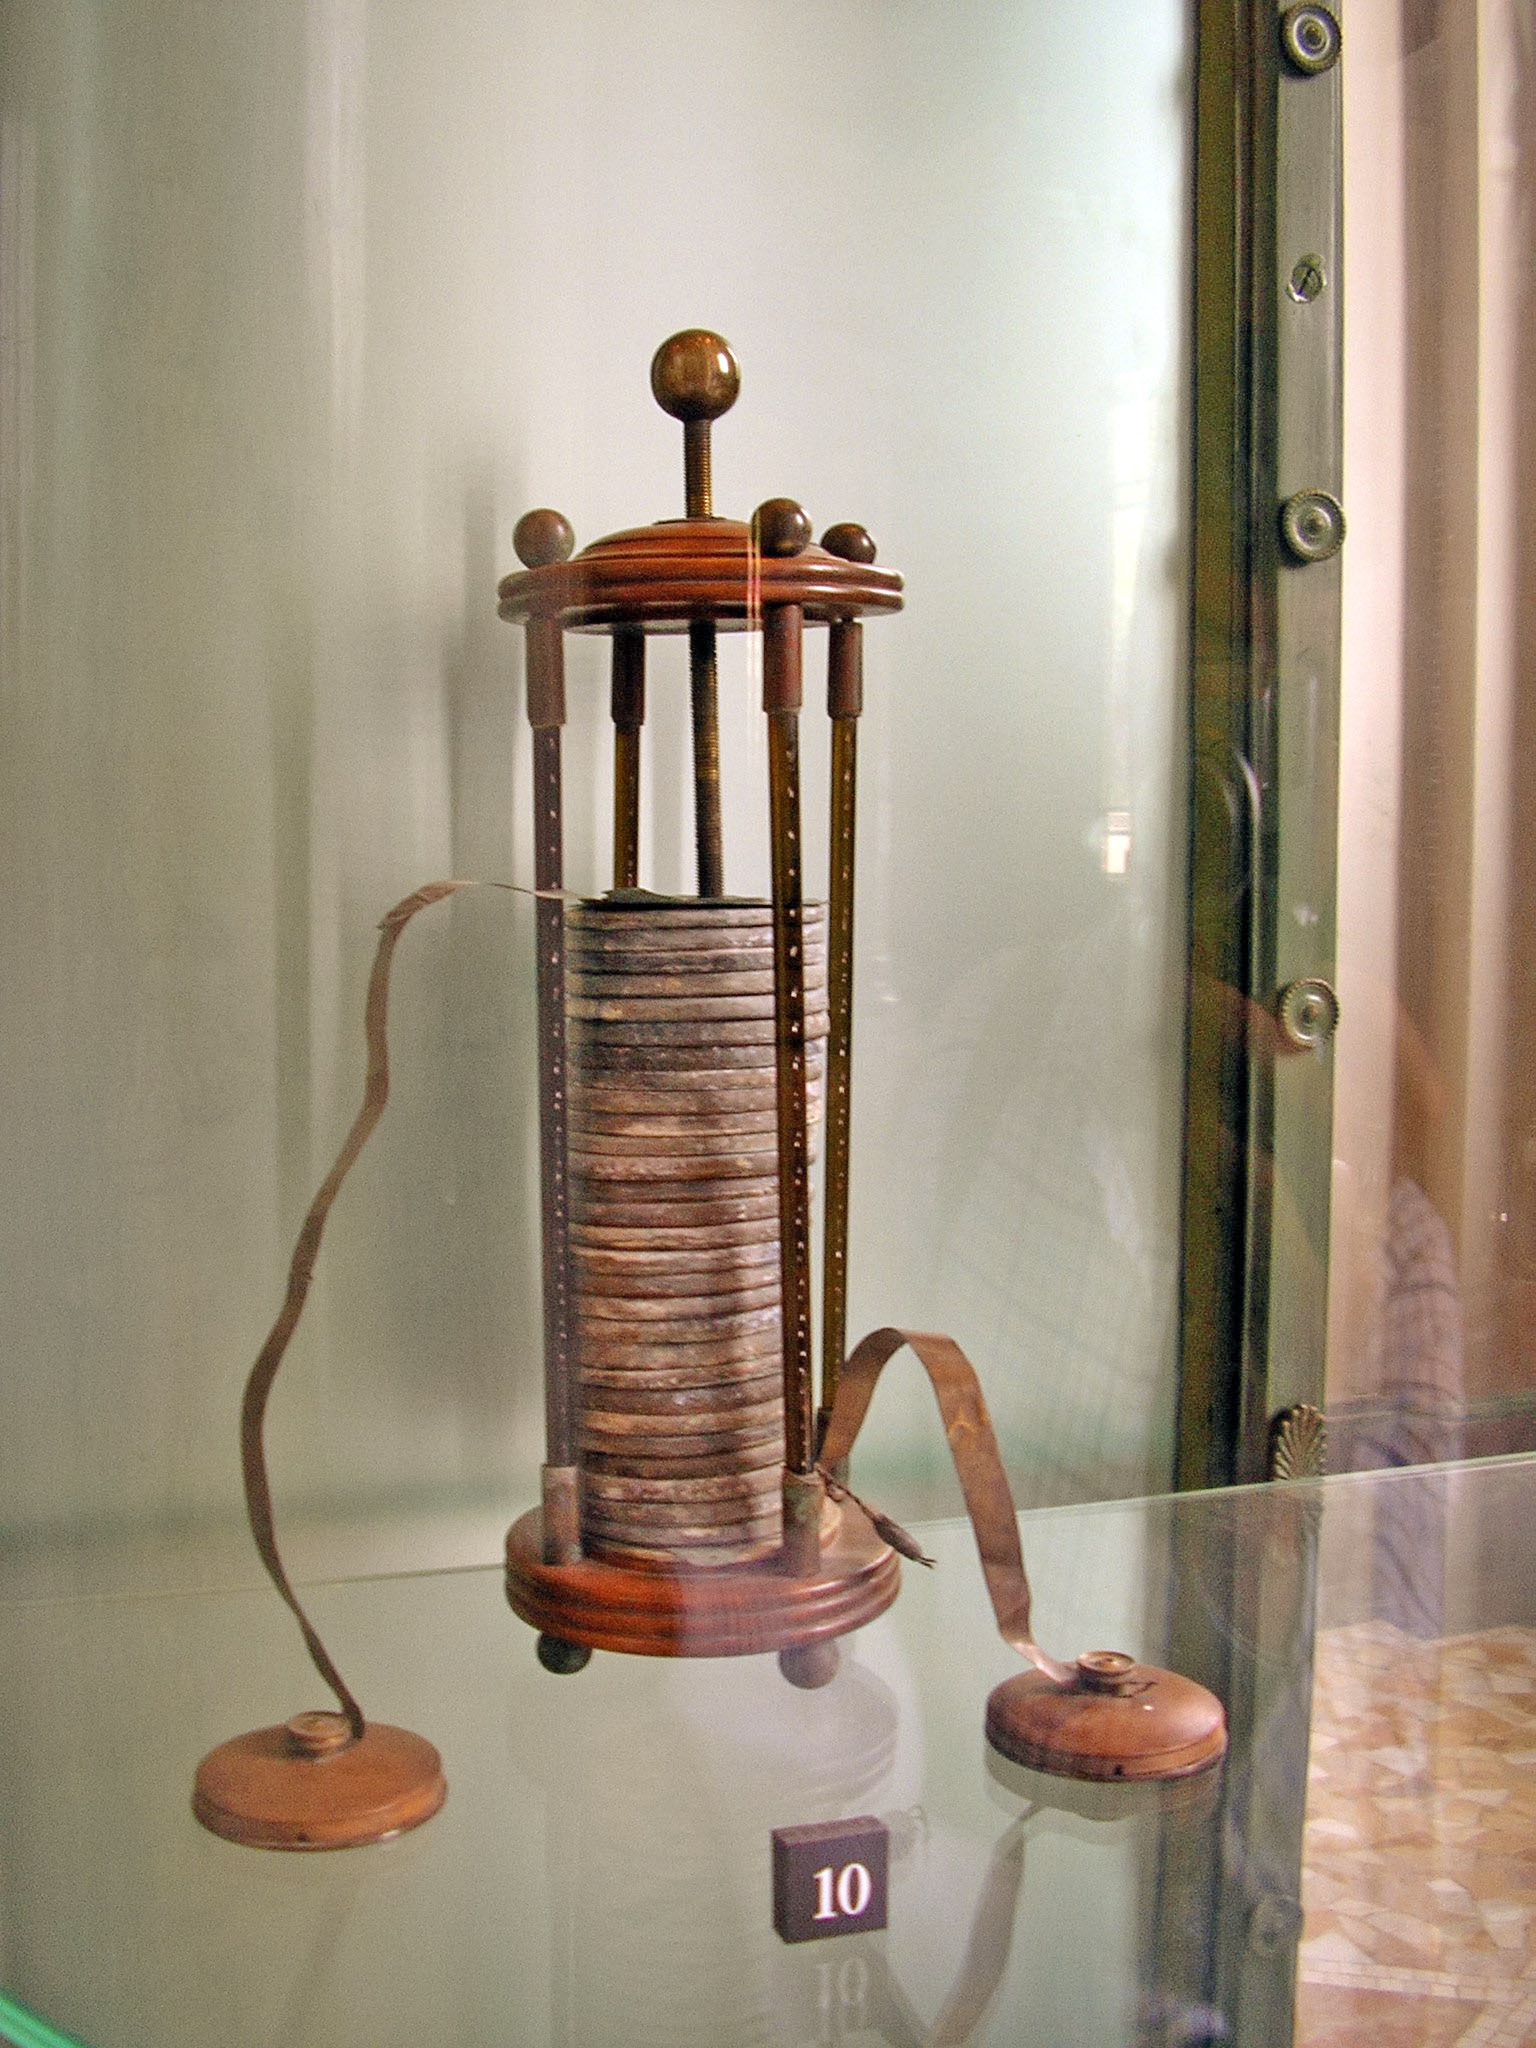
\includegraphics[width=0.24\linewidth]{images/book1/volta-pile.jpg}

{\small Une \omterm{def:g12:cells-and-electrolysis:cell}{pile} de Volta dans un musée. Photo GuidoB, CC BY-SA 3.0.}
\end{omfigure}

\section{La tension d'une pile}

\begin{definition}[Tension à vide]\label{def:g12:cells-and-electrolysis:emf}
La \emph{tension à vide}\index{tension a vide@tension à vide} d'une \omterm{def:g12:cells-and-electrolysis:cell}{pile} est la tension
mesurée entre ses bornes quand elle ne débite aucun courant (circuit
ouvert), à l'aide d'un voltmètre~; elle est positive quand la borne
positive du voltmètre est reliée à la \omterm{def:g12:cells-and-electrolysis:anode}{cathode}.
\end{definition}

\begin{example}[La pile Daniell]\label{ex:g12:cells-and-electrolysis:daniell}
% ledger: e0:Cu, e0:Zn, emf:Daniell
Avec les deux solutions à \qty{1}{mol/L}, la \omterm{def:g12:cells-and-electrolysis:cell}{pile} Daniell donne
\qty{1.10}{V}. La façon de prévoir une telle tension à partir de tables
de potentiels d'électrode est présentée dans le volume de première année
d'université.
\end{example}

\begin{remark}[Pourquoi une pile s'use]\label{rem:g12:cells-and-electrolysis:runs-down}
La réaction de la \omterm{def:g12:cells-and-electrolysis:cell}{pile}, \ce{Zn + Cu^{2+} -> Zn^{2+} + Cu}, a une
constante $K$ très grande. Pendant que la \omterm{def:g12:cells-and-electrolysis:cell}{pile} fonctionne,
$Q = [\ce{Zn^{2+}}]/[\ce{Cu^{2+}}]$
augmente, et la réaction se poursuit tant que $Q < K$. Quand un \omterm{def:g7:chemical-reactions:reactant}{réactif}
est épuisé (le zinc, ou les \omterm{def:g9:ions:ion}{ions} cuivre), le courant s'arrête~: la \omterm{def:g12:cells-and-electrolysis:cell}{pile}
est «~usée~».
\end{remark}

\section{Charge et capacité}

\begin{definition}[Constante de Faraday, capacité]\label{def:g12:cells-and-electrolysis:capacity}
La \emph{constante de Faraday}\index{constante de Faraday} $F$ est la
charge électrique d'une \omterm{def:g10:the-mole:amount}{mole} d'\omterm{def:g9:inside-the-atom:nucleus}{électrons}, $F = N_A e = \qty{96485}{C/mol}$.
La \emph{capacité}\index{capacite@capacité} d'une \omterm{def:g12:cells-and-electrolysis:cell}{pile} est la plus grande charge
électrique qu'elle peut débiter, souvent exprimée en ampères-heures~:
$\qty{1}{A.h} = \qty{3600}{C}$.
\end{definition}

\begin{proposition}[Charge et quantité d'électrons]\label{prop:g12:cells-and-electrolysis:charge}
% ledger: const:F, const:NA, const:e
Un courant d'intensité $I$ qui circule pendant une durée $\Delta t$
transporte la charge
$Q = I\,\Delta t$, soit une quantité d'\omterm{def:g9:inside-the-atom:nucleus}{électrons}
\[
  n(e^-) = \frac{Q}{F} = \frac{I\,\Delta t}{F} .
\]
\end{proposition}

\begin{proof}
Chaque \omterm{def:g9:inside-the-atom:nucleus}{électron} porte la charge élémentaire $e$~; $n$ \omterm{def:g10:the-mole:amount}{moles} d'\omterm{def:g9:inside-the-atom:nucleus}{électrons}
portent $n N_A e = n F$.
\end{proof}

\begin{example}[La capacité d'une pile Daniell]\label{ex:g12:cells-and-electrolysis:capacity}
% ledger: aw:Zn, const:F
L'électrode de zinc contient \qty{6.5}{g} de zinc susceptible de
réagir, soit
$6.5/65.4 = \qty{0.099}{mol}$. Chaque \omterm{def:g7:atoms-and-molecules:atom}{atome} de zinc cède deux
\omterm{def:g9:inside-the-atom:nucleus}{électrons}~:
$n(e^-) = \qty{0.199}{mol}$, donc $Q = 0.199 \times 96485 = \qty{1.9e4}{C}$,
soit environ $\qty{1.9e4}{}/3600 = \qty{5.3}{A.h}$, si les \omterm{def:g9:ions:ion}{ions} cuivre ne
s'épuisent pas avant.
\end{example}

\section{L'électrolyse}

\begin{definition}[Électrolyse, accumulateur]\label{def:g12:cells-and-electrolysis:electrolysis}
Une \emph{électrolyse}\index{electrolyse@électrolyse} est une \omterm{def:g11:redox:reaction}{réaction
d'oxydoréduction} forcée par un générateur électrique, dans le sens
opposé à celui qu'elle prendrait d'elle-même. Un
\emph{accumulateur}\index{accumulateur} est une \omterm{def:g12:cells-and-electrolysis:cell}{pile} rechargeable~:
pendant la charge, le générateur force sa réaction en sens inverse, comme
une électrolyse.
\end{definition}

\begin{inthelab}[L'électrolyse de l'eau]
Deux électrodes plongent dans de l'eau rendue conductrice par un peu de
sulfate de sodium, chacune sous un tube à essai retourné rempli de la
solution. Avec un générateur de quelques volts, des bulles montent des
deux électrodes~: à la \omterm{def:g12:cells-and-electrolysis:anode}{cathode} (reliée à la borne $-$), du dihydrogène,
à l'\omterm{def:g12:cells-and-electrolysis:anode}{anode}, du dioxygène, avec deux fois plus du premier gaz que du
second. Une allumette enflammée produit une petite détonation dans le
premier gaz~; une bûchette incandescente se rallume dans le second.
\end{inthelab}

\begin{omfigure}
\begin{tikzpicture}[font=\small, scale=1.2]
  % a trough of water, two inverted tubes standing in it
  \fill[omWater] (-1.4,0) rectangle (1.4,1.1);
  \foreach \x/\g in {-0.6/1.2, 0.6/0.6} {
    \fill[omWater] (\x-0.18,0.3) rectangle (\x+0.18,2.9);
    \fill[white] (\x-0.18,{2.9-\g}) rectangle (\x+0.18,2.9);
    \fill[white] (\x,2.9) circle (0.18);
    \draw[om glass] (\x-0.18,0.3) -- (\x-0.18,2.9) arc[start angle=180, end angle=0, radius=0.18] -- (\x+0.18,0.3);
  }
  \draw[om glass] (-1.5,1.25) -- (-1.4,1.15) -- (-1.4,0) -- (1.4,0) -- (1.4,1.15) -- (1.5,1.25);
  \fill[black!55] (-0.65,0) rectangle (-0.55,0.6);
  \fill[black!55] (0.55,0) rectangle (0.65,0.6);
  \node[draw, fill=white, minimum width=1.6cm, minimum height=0.45cm, font=\footnotesize] (g) at (0,-0.75) {générateur};
  \draw[black!70, thick] (-0.6,0) -- (-0.6,0 |- g.north);
  \draw[black!70, thick] (0.6,0) -- (0.6,0 |- g.north);
  \node[font=\footnotesize] at (-0.78,-0.3) {$-$};
  \node[font=\footnotesize] at (0.78,-0.3) {$+$};
  \node[anchor=east, align=right] at (-0.95,2.5) {dihydrogène\\ (cathode)};
  \node[anchor=west, align=left] at (0.95,2.5) {dioxygène\\ (anode)};
\end{tikzpicture}

{\small L'\omterm{def:g12:cells-and-electrolysis:electrolysis}{électrolyse} de l'eau~: il se rassemble deux fois plus de
dihydrogène que de dioxygène au-dessus des électrodes.}
\end{omfigure}


\begin{example}[L'eau décomposée]\label{ex:g12:cells-and-electrolysis:water}
À la \omterm{def:g12:cells-and-electrolysis:anode}{cathode}~: \ce{2H2O + 2e- -> H2 + 2OH-}~; à l'\omterm{def:g12:cells-and-electrolysis:anode}{anode}~:
\ce{6H2O -> O2 + 4H3O+ + 4e-}. Pour quatre \omterm{def:g9:inside-the-atom:nucleus}{électrons}, on obtient deux
\omterm{def:g7:atoms-and-molecules:molecule}{molécules} de dihydrogène et une de dioxygène, tandis que les \omterm{def:g9:ions:ion}{ions}
\ce{H3O+} et \ce{OH-} formés aux deux électrodes se recombinent en eau~:
au total,
\ce{2H2O -> 2H2 + O2}, l'inverse de la \omterm{def:g4:what-a-fire-needs:burning}{combustion} du dihydrogène, qui
a besoin d'énergie pour se produire.
\end{example}

\begin{method}[Masse déposée par une électrolyse]\label{met:g12:cells-and-electrolysis:mass}
\begin{enumerate}
  \item Écrire la \omterm{def:g11:redox:couple}{demi-équation} à l'électrode où le \omterm{def:g9:periodic-table-first-look:metal}{métal} se forme, par
        exemple \ce{Cu^{2+} + 2e- -> Cu}.
  \item Calculer la charge $Q = I \Delta t$ et $n(e^-) = Q/F$.
  \item Diviser par le nombre d'\omterm{def:g9:inside-the-atom:nucleus}{électrons} par \omterm{def:g7:atoms-and-molecules:atom}{atome}~: $n(\ce{Cu}) =
        n(e^-)/2$~; puis $m = n \times M$.
\end{enumerate}
\end{method}


\begin{example}[Le raffinage du cuivre]\label{ex:g12:cells-and-electrolysis:refining}
% ledger: aw:Cu, const:F
Le cuivre impur sortant de la fonderie constitue l'\omterm{def:g12:cells-and-electrolysis:anode}{anode} d'une cuve
d'\omterm{def:g12:cells-and-electrolysis:electrolysis}{électrolyse} contenant une solution de sulfate de cuivre, et une fine
feuille de cuivre pur la \omterm{def:g12:cells-and-electrolysis:anode}{cathode}. À l'\omterm{def:g12:cells-and-electrolysis:anode}{anode}, le cuivre \omterm{def:g2:mixing-and-dissolving:dissolve}{se dissout},
\ce{Cu -> Cu^{2+} + 2e-}~; à la \omterm{def:g12:cells-and-electrolysis:anode}{cathode}, du cuivre pur se dépose,
\ce{Cu^{2+} + 2e- -> Cu}~; les impuretés tombent au fond ou restent en
solution. Un courant de \qty{100}{A} pendant
\qty{24}{h} transporte $Q = 100 \times 86400 = \qty{8.64e6}{C}$, soit
$n(e^-) = \qty{89.5}{mol}$, ce qui dépose $89.5/2 = \qty{44.8}{mol}$ de
cuivre~: \qty{2.84}{kg}.
\end{example}

\begin{omfigure}
\begin{tikzpicture}[font=\small, scale=1.25]
  \pic[transform shape] at (0,0) {beaker={0.75}{cyan!70!blue!35}};
  \pic[transform shape] (an) at (-0.4,0.2) {electrode={orange!40!brown!80!black}};
  \pic[transform shape] (ca) at (0.4,0.2) {electrode={orange!80!brown}};
  \foreach \p in {(-0.6,0.08),(-0.5,0.12),(-0.3,0.07),(-0.2,0.1)} \fill[black!55] \p circle (0.03);
  \node[draw, fill=white, font=\footnotesize, minimum width=1.6cm] (g) at (0,3.4) {générateur};
  \draw[black!70, thick] (an-top) -- (an-top |- g.south);
  \draw[black!70, thick] (ca-top) -- (ca-top |- g.south);
  \node[font=\footnotesize] at (-0.58,2.95) {$+$};
  \node[font=\footnotesize] at (0.58,2.95) {$-$};
  \draw[omProp, thick, <-] (-0.55,1.2) -- (-1.6,1.6) node[left, align=right, text=black] {anode en cuivre\\ impur~: se dissout};
  \draw[omProp, thick, <-] (0.55,1.2) -- (1.6,1.6) node[right, align=left, text=black] {cathode en cuivre\\ pur~: grossit};
  \draw[omProp, thick, <-] (-0.35,0.1) -- (-1.6,0.3) node[left, text=black] {impuretés};
\end{tikzpicture}

{\small Le raffinage du cuivre par \omterm{def:g12:cells-and-electrolysis:electrolysis}{électrolyse}~: le cuivre passe de
l'\omterm{def:g12:cells-and-electrolysis:anode}{anode} impure à la \omterm{def:g12:cells-and-electrolysis:anode}{cathode} pure à travers la solution.}
\end{omfigure}

\section{Piles, accumulateurs et piles à combustible}

Toute \omterm{def:g12:cells-and-electrolysis:cell}{pile} du commerce est une \omterm{def:g12:cells-and-electrolysis:cell}{pile} au sens de ce chapitre, toute
batterie rechargeable un \omterm{def:g12:cells-and-electrolysis:electrolysis}{accumulateur}. L'\omterm{def:g12:cells-and-electrolysis:electrolysis}{accumulateur} au plomb d'une
voiture fonctionne avec du plomb, de l'oxyde de plomb et de l'acide
sulfurique~; l'\omterm{def:g12:cells-and-electrolysis:electrolysis}{accumulateur} \omterm{def:g9:ions:ion}{lithium-ion} d'un téléphone fait passer des
\omterm{def:g9:ions:ion}{ions} lithium entre deux électrodes, l'une en graphite et l'autre en
oxyde métallique, à travers un électrolyte liquide ou polymère, tandis
que les \omterm{def:g9:inside-the-atom:nucleus}{électrons} parcourent le circuit extérieur. Une \omterm{def:g12:cells-and-electrolysis:cell}{pile} à
\omterm{def:g4:what-a-fire-needs:fuel}{combustible} est une \omterm{def:g12:cells-and-electrolysis:cell}{pile} dont les \omterm{def:g7:chemical-reactions:reactant}{réactifs} sont apportés en continu~:
une \omterm{def:g12:cells-and-electrolysis:cell}{pile} à hydrogène met en œuvre la réaction \ce{2H2 + O2 -> 2H2O},
l'inverse de l'\omterm{def:g12:cells-and-electrolysis:electrolysis}{électrolyse} de l'eau, et fournit de l'électricité et de
l'eau. Le dihydrogène produit par \omterm{def:g12:cells-and-electrolysis:electrolysis}{électrolyse} avec de l'électricité
d'origine éolienne ou solaire, puis utilisé dans des \omterm{def:g12:cells-and-electrolysis:cell}{piles} à
\omterm{def:g4:what-a-fire-needs:fuel}{combustible}, est un moyen de stocker cette électricité.

\begin{omfigure}
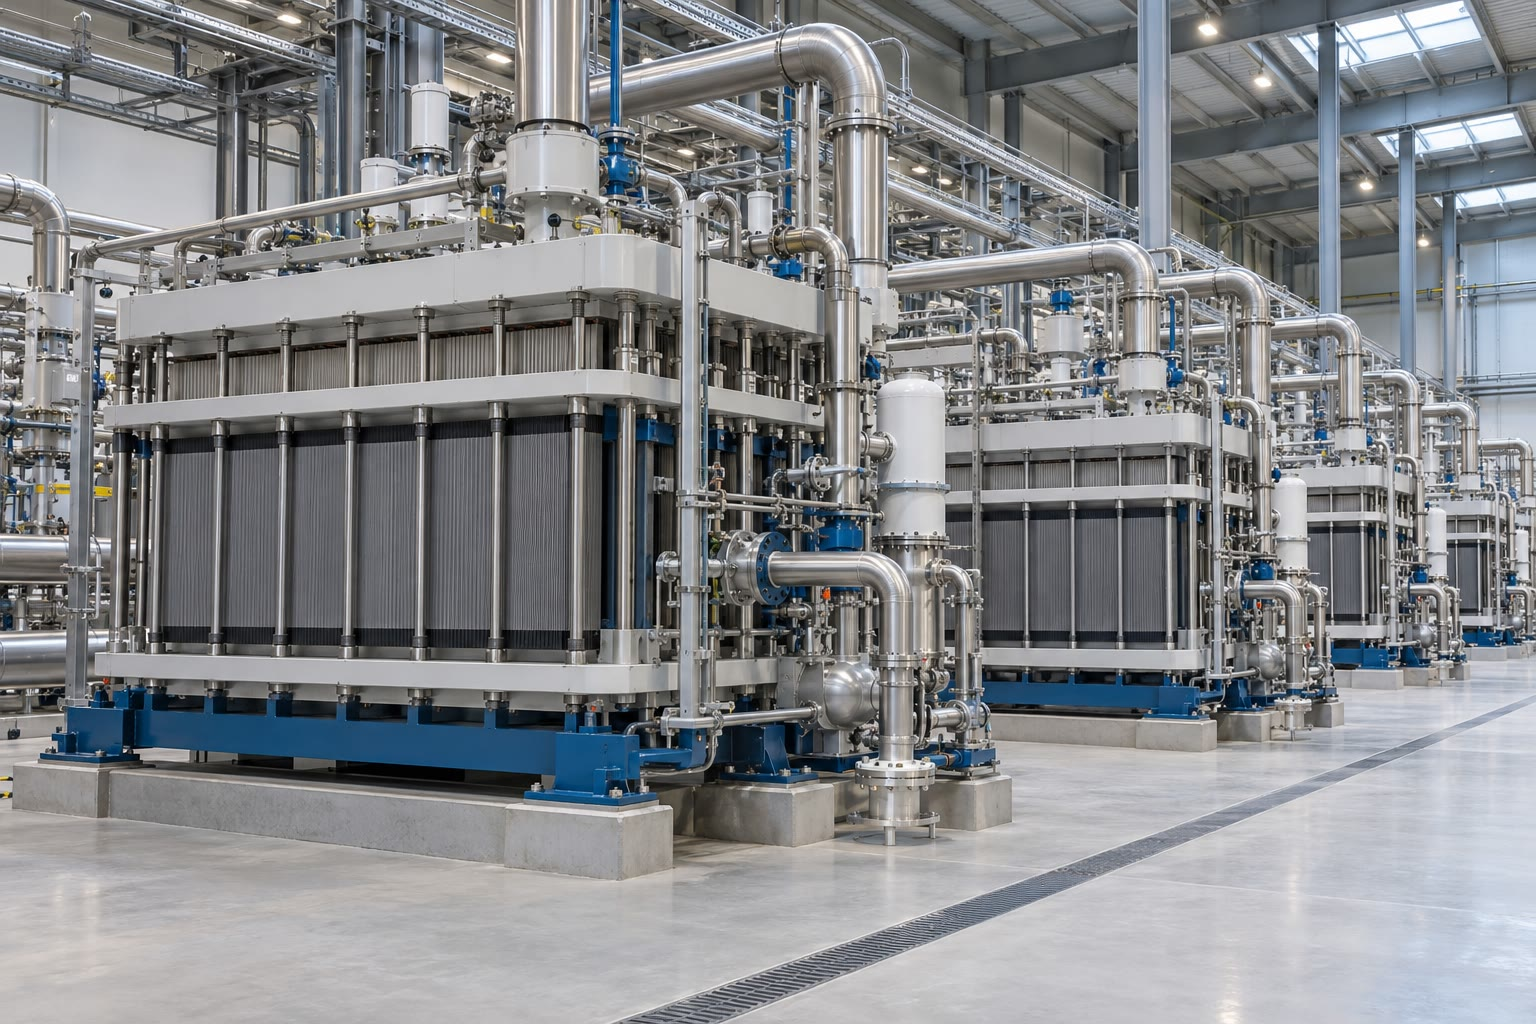
\includegraphics[width=0.48\linewidth]{images/book1/ai/g12-electrolyser-hall.jpg}

{\small Un hall d'électrolyseurs~: l'eau y est décomposée en dihydrogène
et en dioxygène.}
\end{omfigure}

\section{Exercices}

\begin{exercise}[$\star$]\label{exo:g12:cells-and-electrolysis:1}
Dans la \omterm{def:g12:cells-and-electrolysis:cell}{pile} Daniell, quelle électrode est l'\omterm{def:g12:cells-and-electrolysis:anode}{anode}~? La \omterm{def:g12:cells-and-electrolysis:anode}{cathode}~?
Écrire la \omterm{def:g11:redox:couple}{demi-équation} à chacune.
\end{exercise}

\begin{exercise}[$\star$]\label{exo:g12:cells-and-electrolysis:2}
Un courant de \qty{0.20}{A} circule pendant \qty{30}{min}. Calculer la
charge transportée et la quantité d'\omterm{def:g9:inside-the-atom:nucleus}{électrons}.
\end{exercise}

\begin{exercise}[$\star$]\label{exo:g12:cells-and-electrolysis:3}
Quel est le rôle du \omterm{def:g12:cells-and-electrolysis:cell}{pont salin}~? Que se passe-t-il si on le retire~?
\end{exercise}

\begin{exercise}[$\star$]\label{exo:g12:cells-and-electrolysis:4}
Convertir une \omterm{def:g12:cells-and-electrolysis:capacity}{capacité} de \qty{2.5}{A.h} en coulombs.
\end{exercise}

\begin{exercise}[$\star$]\label{exo:g12:cells-and-electrolysis:5}
Dans une \omterm{def:g12:cells-and-electrolysis:electrolysis}{électrolyse}, la réaction est-elle spontanée~? Qu'est-ce qui
fournit l'énergie~?
\end{exercise}

\begin{exercise}[$\star\star$]\label{exo:g12:cells-and-electrolysis:6}
Une \omterm{def:g12:cells-and-electrolysis:cell}{pile} est constituée d'une électrode d'argent dans une solution de
nitrate d'argent et d'une électrode de cuivre dans une solution de
sulfate de cuivre. Le voltmètre montre que les \omterm{def:g9:inside-the-atom:nucleus}{électrons} sortent par le
cuivre. Écrire les \omterm{def:g11:redox:couple}{demi-équations}, nommer l'\omterm{def:g12:cells-and-electrolysis:anode}{anode} et la \omterm{def:g12:cells-and-electrolysis:anode}{cathode}, et
donner la réaction globale.
\end{exercise}

\begin{exercise}[$\star\star$]\label{exo:g12:cells-and-electrolysis:7}
Une \omterm{def:g12:cells-and-electrolysis:cell}{pile} de montre débite \qty{10}{\micro A} en continu pendant trois
ans. Quelle est sa \omterm{def:g12:cells-and-electrolysis:capacity}{capacité} en \si{mA.h}~?
\end{exercise}

\begin{exercise}[$\star\star$]\label{exo:g12:cells-and-electrolysis:8}
On argente une cuillère avec un courant de \qty{0.50}{A} pendant
\qty{40}{min}, \ce{Ag+ + e- -> Ag}. Quelle masse d'argent se dépose-t-il~?
\end{exercise}

\begin{exercise}[$\star\star$]\label{exo:g12:cells-and-electrolysis:9}
Sur la figure de la \omterm{def:g12:cells-and-electrolysis:cell}{pile} Daniell, donner le sens du courant dans le fil,
et le sens de déplacement des \omterm{def:g9:ions:ion}{ions} \ce{K+} et \ce{NO3-} du pont.
\end{exercise}

\begin{exercise}[$\star\star$]\label{exo:g12:cells-and-electrolysis:10}
Comparer une \omterm{def:g12:cells-and-electrolysis:cell}{pile} et une \omterm{def:g12:cells-and-electrolysis:electrolysis}{électrolyse}~: le signe de l'\omterm{def:g12:cells-and-electrolysis:anode}{anode}, le sens de
la réaction, la conversion d'énergie.
\end{exercise}

\begin{exercise}[$\star\star$]\label{exo:g12:cells-and-electrolysis:11}
Lors de l'\omterm{def:g12:cells-and-electrolysis:electrolysis}{électrolyse} de l'eau, on recueille \qty{24}{mL} de
dihydrogène. Quel volume de dioxygène recueille-t-on dans le même
temps~? Pourquoi~?
\end{exercise}

\begin{exercise}[$\star\star\star$]\label{exo:g12:cells-and-electrolysis:12}
Une \omterm{def:g12:cells-and-electrolysis:cell}{pile} Daniell contient \qty{5.0}{g} de zinc et \qty{100}{mL} de
sulfate de cuivre à \qty{0.50}{mol/L}. Quel \omterm{def:g7:chemical-reactions:reactant}{réactif} s'épuise en
premier~? Quelle est la \omterm{def:g12:cells-and-electrolysis:capacity}{capacité} de la \omterm{def:g12:cells-and-electrolysis:cell}{pile}~? Pendant combien de temps
peut-elle débiter \qty{50}{mA}~?
\end{exercise}

\begin{exercise}[$\star\star\star$]\label{exo:g12:cells-and-electrolysis:13}
Une \omterm{def:g12:cells-and-electrolysis:cell}{pile} de \qty{1.5}{V} débite \qty{2.0}{A.h}. Calculer l'énergie
qu'elle stocke ($E = Q U$), en joules et en wattheures.
\end{exercise}

\begin{exercise}[$\star\star\star$]\label{exo:g12:cells-and-electrolysis:14}
On \omterm{def:g12:cells-and-electrolysis:electrolysis}{électrolyse} de l'eau avec \qty{2.0}{A} pendant \qty{1.0}{h}. Calculer
les quantités, puis les volumes à \qty{20}{\celsius}
($V_m = \qty{24.1}{L/mol}$),
de dihydrogène et de dioxygène produits.
\end{exercise}

\begin{exercise}[$\star\star\star$]\label{exo:g12:cells-and-electrolysis:15}
Lors du raffinage du cuivre, l'\omterm{def:g12:cells-and-electrolysis:anode}{anode} perd \qty{3.00}{kg} de matière
tandis que la \omterm{def:g12:cells-and-electrolysis:anode}{cathode} gagne \qty{2.84}{kg} de cuivre. Quel est le
pourcentage de cuivre dans l'\omterm{def:g12:cells-and-electrolysis:anode}{anode} impure, en supposant que seul le
cuivre est oxydé à l'\omterm{def:g12:cells-and-electrolysis:anode}{anode} et que les impuretés tombent simplement au
fond~?
\end{exercise}

\section{Problème~: la batterie du téléphone}

\begin{problem}[{Problème du week-end --- quelle masse de lithium fait la
navette entre les électrodes d'une batterie de téléphone de
\qty{4000}{mA.h}~?}]
\label{pb:g12:cells-and-electrolysis:1}
% ledger: const:F, const:NA, aw:Li, dch:CH4, aw:C, aw:H
La batterie d'un téléphone porte l'indication «~\qty{3.7}{V},
\qty{4000}{mA.h}~». Dans une description simplifiée, pendant la
décharge, chaque \omterm{def:g7:atoms-and-molecules:atom}{atome} de lithium stocké dans l'électrode de graphite
cède un \omterm{def:g9:inside-the-atom:nucleus}{électron} et part sous forme d'\omterm{def:g9:ions:ion}{ion} lithium,
\ce{Li -> Li+ + e-}~; l'\omterm{def:g9:ions:ion}{ion} traverse l'électrolyte et est accueilli par
l'électrode d'oxyde métallique, qui gagne un \omterm{def:g9:inside-the-atom:nucleus}{électron} au même moment.

\medskip
\noindent\textbf{Partie I --- La \omterm{def:g12:cells-and-electrolysis:cell}{pile}.}
\begin{enumerate}
  \item Pendant la décharge, l'électrode de graphite est-elle l'\omterm{def:g12:cells-and-electrolysis:anode}{anode} ou
        la \omterm{def:g12:cells-and-electrolysis:anode}{cathode}~? Pourquoi~?
  \item Quelle est la borne négative~?
  \item Dans quel sens les \omterm{def:g9:inside-the-atom:nucleus}{électrons} circulent-ils à travers le
        téléphone~? Et les \omterm{def:g9:ions:ion}{ions} lithium à l'intérieur de la batterie~?
  \item Pourquoi cette \omterm{def:g12:cells-and-electrolysis:cell}{pile} est-elle un \omterm{def:g12:cells-and-electrolysis:electrolysis}{accumulateur}~?
\end{enumerate}

\medskip
\noindent\textbf{Partie II --- La charge.}
\begin{enumerate}[resume]
  \item Convertir \qty{4000}{mA.h} en ampères-heures, puis en coulombs.
  \item Calculer la quantité d'\omterm{def:g9:inside-the-atom:nucleus}{électrons} que représente cette charge.
  \item Combien d'\omterm{def:g9:inside-the-atom:nucleus}{électrons} cela fait-il~?
  \item Le téléphone consomme en moyenne \qty{0.25}{A}. Combien de temps
        dure une batterie pleine~?
  \item L'écran affiche 20~\%. Quelle charge, en coulombs, reste-t-il~?
\end{enumerate}

\medskip
\noindent\textbf{Partie III --- L'énergie.}
\begin{enumerate}[resume]
  \item Calculer l'énergie stockée, $E = Q U$, en joules.
  \item La convertir en wattheures.
  \item La comparer à l'énergie libérée par la \omterm{def:g4:what-a-fire-needs:burning}{combustion} de
        \qty{1}{g} de méthane
        (\qty{55.7}{kJ}).
  \item Combien de charges complètes \qty{1}{kW.h} d'électricité
        donne-t-il, si aucune énergie n'était perdue~?
\end{enumerate}

\medskip
\noindent\textbf{Partie IV --- La recharge.}
\begin{enumerate}[resume]
  \item Pendant la charge, quelle réaction a lieu à l'électrode de
        graphite~? Est-ce une \omterm{def:g11:redox:oxidation}{oxydation} ou une \omterm{def:g11:redox:oxidation}{réduction}~?
  \item Pourquoi la recharge est-elle une \omterm{def:g12:cells-and-electrolysis:electrolysis}{électrolyse}~?
  \item Le chargeur débite \qty{2.0}{A}. Combien de temps dure au minimum
        une recharge complète~?
  \item Quelle quantité d'\omterm{def:g9:ions:ion}{ions} lithium traverse l'électrolyte pendant une
        charge complète~?
  \item Calculer leur masse.
  \item Donner la réponse finale~: quelle masse de lithium fait la
        navette entre les électrodes au cours d'une charge complète~?
\end{enumerate}
\end{problem}
